\documentclass{article}
\usepackage[table,xcdraw]{xcolor}
\usepackage{graphicx}
\usepackage{listings}
\usepackage{hyperref}
\usepackage{pdfpages}
\usepackage{csvsimple}
\usepackage{float}
\makeatletter
\newcommand\urlfootnote@[1]{\footnote{\url@{#1}}}
\DeclareRobustCommand{\urlfootnote}{\hyper@normalise\urlfootnote@}
\makeatother

\begin{document}
\title{Neural Networks Assignment 1}
\author{Group 35}
\maketitle
\lstset{
  basicstyle=\ttfamily,
  keywordstyle=\bfseries,
  language=Java,
  frame=single,
  aboveskip=11pt,
  belowskip=11pt,
  breaklines=true,
  breakatwhitespace=false,
  showspaces=false,
  showstringspaces=false,
  numbers=left,
  stepnumber=1,    
  firstnumber=1,
  numberfirstline=true
}
\section{Excercise 1: Image Distance}
\label{a1}

This is the table for our cloud distances.

% Please add the following required packages to your document preamble:
% \usepackage[table,xcdraw]{xcolor}
% If you use beamer only pass "xcolor=table" option, i.e. \documentclass[xcolor=table]{beamer}
\begin{table}[]
	\centering
	\label{my-label}
	\begin{tabular}{lllllllllll}
		                      & 0                                                 & 1                                                 & 2                                                 & 3                                                 & 4                                                 & 5                                                 & 6                                                 & 7                                                 & 8                                                 & 9                                                 \\ \cline{2-11} 
		\multicolumn{1}{l|}{0} & \multicolumn{1}{l|}{\cellcolor[HTML]{C0C0C0}0.00} & \multicolumn{1}{l|}{14.45}                        & \multicolumn{1}{l|}{9.33}                         & \multicolumn{1}{l|}{9.14}                         & \multicolumn{1}{l|}{10.77}                        & \multicolumn{1}{l|}{7.52}                         & \multicolumn{1}{l|}{8.15}                         & \multicolumn{1}{l|}{11.86}                        & \multicolumn{1}{l|}{9.91}                         & \multicolumn{1}{l|}{11.49}                        \\ \cline{2-11} 
		\multicolumn{1}{l|}{1} & \multicolumn{1}{l|}{14.45}                        & \multicolumn{1}{l|}{\cellcolor[HTML]{C0C0C0}0.00} & \multicolumn{1}{l|}{10.13}                        & \multicolumn{1}{l|}{11.73}                        & \multicolumn{1}{l|}{10.17}                        & \multicolumn{1}{l|}{11.12}                        & \multicolumn{1}{l|}{10.61}                        & \multicolumn{1}{l|}{10.74}                        & \multicolumn{1}{l|}{10.09}                        & \multicolumn{1}{l|}{9.93}                         \\ \cline{2-11} 
		\multicolumn{1}{l|}{2} & \multicolumn{1}{l|}{9.33}                         & \multicolumn{1}{l|}{10.13}                        & \multicolumn{1}{l|}{\cellcolor[HTML]{C0C0C0}0.00} & \multicolumn{1}{l|}{8.18}                         & \multicolumn{1}{l|}{7.93}                         & \multicolumn{1}{l|}{7.91}                         & \multicolumn{1}{l|}{7.33}                         & \multicolumn{1}{l|}{8.87}                         & \multicolumn{1}{l|}{7.08}                         & \multicolumn{1}{l|}{8.89}                         \\ \cline{2-11} 
		\multicolumn{1}{l|}{3} & \multicolumn{1}{l|}{9.14}                         & \multicolumn{1}{l|}{11.73}                        & \multicolumn{1}{l|}{8.18}                         & \multicolumn{1}{l|}{\cellcolor[HTML]{C0C0C0}0.00} & \multicolumn{1}{l|}{9.09}                         & \multicolumn{1}{l|}{6.12}                         & \multicolumn{1}{l|}{9.30}                         & \multicolumn{1}{l|}{8.92}                         & \multicolumn{1}{l|}{7.02}                         & \multicolumn{1}{l|}{8.35}                         \\ \cline{2-11} 
		\multicolumn{1}{l|}{4} & \multicolumn{1}{l|}{10.77}                        & \multicolumn{1}{l|}{10.17}                        & \multicolumn{1}{l|}{7.93}                         & \multicolumn{1}{l|}{9.09}                         & \multicolumn{1}{l|}{\cellcolor[HTML]{C0C0C0}0.00} & \multicolumn{1}{l|}{8.00}                         & \multicolumn{1}{l|}{8.78}                         & \multicolumn{1}{l|}{7.58}                         & \multicolumn{1}{l|}{7.38}                         & \multicolumn{1}{l|}{6.01}                         \\ \cline{2-11} 
		\multicolumn{1}{l|}{5} & \multicolumn{1}{l|}{7.52}                         & \multicolumn{1}{l|}{11.12}                        & \multicolumn{1}{l|}{7.91}                         & \multicolumn{1}{l|}{6.12}                         & \multicolumn{1}{l|}{8.00}                         & \multicolumn{1}{l|}{\cellcolor[HTML]{C0C0C0}0.00} & \multicolumn{1}{l|}{6.70}                         & \multicolumn{1}{l|}{9.21}                         & \multicolumn{1}{l|}{6.97}                         & \multicolumn{1}{l|}{8.26}                         \\ \cline{2-11} 
		\multicolumn{1}{l|}{6} & \multicolumn{1}{l|}{8.15}                         & \multicolumn{1}{l|}{10.61}                        & \multicolumn{1}{l|}{7.33}                         & \multicolumn{1}{l|}{9.30}                         & \multicolumn{1}{l|}{8.78}                         & \multicolumn{1}{l|}{6.70}                         & \multicolumn{1}{l|}{\cellcolor[HTML]{C0C0C0}0.00} & \multicolumn{1}{l|}{10.89}                        & \multicolumn{1}{l|}{8.59}                         & \multicolumn{1}{l|}{10.44}                        \\ \cline{2-11} 
		\multicolumn{1}{l|}{7} & \multicolumn{1}{l|}{11.86}                        & \multicolumn{1}{l|}{10.74}                        & \multicolumn{1}{l|}{8.87}                         & \multicolumn{1}{l|}{8.92}                         & \multicolumn{1}{l|}{7.58}                         & \multicolumn{1}{l|}{9.21}                         & \multicolumn{1}{l|}{10.89}                        & \multicolumn{1}{l|}{\cellcolor[HTML]{C0C0C0}0.00} & \multicolumn{1}{l|}{8.47}                         & \multicolumn{1}{l|}{5.43}                         \\ \cline{2-11} 
		\multicolumn{1}{l|}{8} & \multicolumn{1}{l|}{9.91}                         & \multicolumn{1}{l|}{10.09}                        & \multicolumn{1}{l|}{7.08}                         & \multicolumn{1}{l|}{7.02}                         & \multicolumn{1}{l|}{7.38}                         & \multicolumn{1}{l|}{6.97}                         & \multicolumn{1}{l|}{8.59}                         & \multicolumn{1}{l|}{8.47}                         & \multicolumn{1}{l|}{\cellcolor[HTML]{C0C0C0}0.00} & \multicolumn{1}{l|}{6.40}                         \\ \cline{2-11} 
		\multicolumn{1}{l|}{9} & \multicolumn{1}{l|}{11.49}                        & \multicolumn{1}{l|}{9.93}                         & \multicolumn{1}{l|}{8.89}                         & \multicolumn{1}{l|}{8.35}                         & \multicolumn{1}{l|}{6.01}                         & \multicolumn{1}{l|}{8.26}                         & \multicolumn{1}{l|}{10.44}                        & \multicolumn{1}{l|}{5.43}                         & \multicolumn{1}{l|}{6.40}                         & \multicolumn{1}{l|}{\cellcolor[HTML]{C0C0C0}0.00} \\ \cline{2-11} 	
	\end{tabular}
	\caption{Cloud distances for the digit 0 - 9}
\end{table}

After calculating the distances between the different classes the most difficult digits to separate from each other are: \[ 7 \rightarrow 9; 4 \rightarrow 9; 3 \rightarrow 5; 9 \rightarrow 8\]

This can be concluded by looking at the distance values. The lowest and hence most similar values we found were 5.43, 6.01, 6.12 and 6.4.
These values were for classifying 7 to 9, 4 to 9, 3 to 5 and 9 to 8.
This does make sense given that a 9 can be, if written by hand, sometimes hard to distinguish from a 7, 4 or 5.


\section{Excercise 2}
\subsection{Confusion Matrix Training and Test Set}
%Which digits were most difficult to classify correctly?%
%Describe your findings. Compare performance of your classifier on the train and test sets. %
The confusion matrices can be found in Figure \ref{fig:cftrain} for the training set and in Figure \ref{fig:cftest} for the testing set.
For the training set (Figure \ref{fig:cftrain}) the number 5 and 4 are most difficult to be classified. Very close in error rates and also harder to identify are 0, 2, 5, 6, 7, 8, 9. The only number with full accuracy is 1. This is quite surprising given that 1 and 7 sometimes look quite alike.

For the testing set (Figure \ref{fig:cftest}) the number 2 is most difficult to classify. Followed by 8, 0, 9, 7 and 3. Also here we have full accuracy for the digit 1.


\begin{figure}[H]
\centering
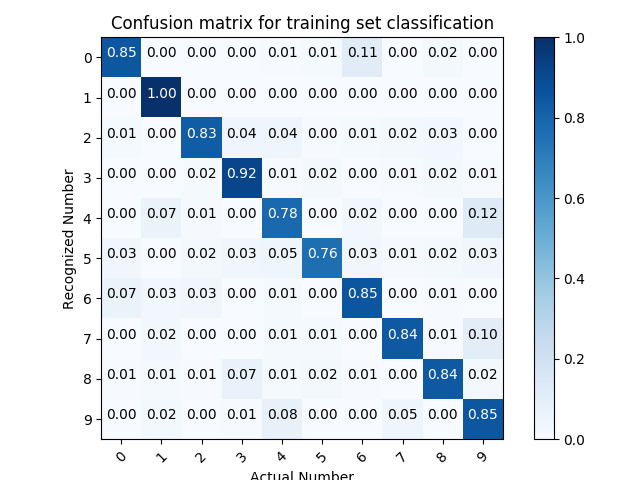
\includegraphics[width=0.9\linewidth]{img/cftrain.png}
\caption{Confusion Matrix visualized for training set}
\label{fig:cftrain}
\end{figure}
\begin{figure}[H]
\centering
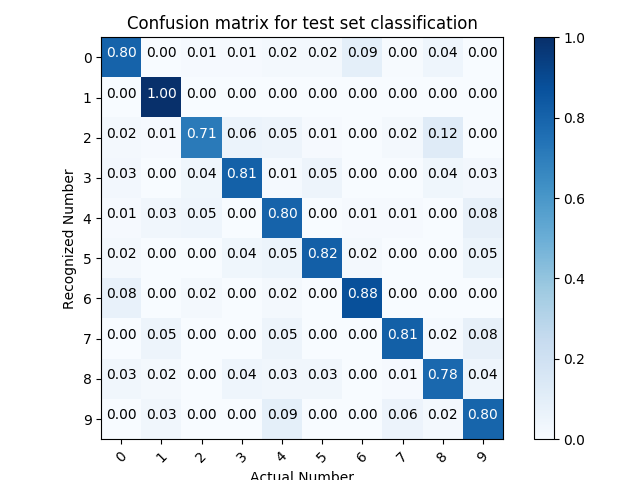
\includegraphics[width=0.9\linewidth]{img/cftest.png}
\caption{Confusion Matrix visualized for test set}
\label{fig:cftest}
\end{figure}

\subsection{Comparison to expectations from A1}
%How do the results compare to the observations you’ve made in Step 1? How would you explain it?%
When comparing our findings with the expectations build up in Excercise 1 (see Section \ref{a1}) the occurred misclassifications are quite different.
If we look at the confusion matrix of the training set our expectations are mostly met. This is because here the  most often misclassified numbers are 4 $\rightarrow$ 9, 7 $\rightarrow$ 9 and 4 $\rightarrow$ 6.
For the test set however this does not prove to be true. Here the most often misclassified numbers are 2 $\rightarrow$ 8, 0 $\rightarrow$ 6 and 9 $\rightarrow$ 4.

This difference could be explained by the amount of actual sample numbers per digit in the classified set.
And of course overfitting might also play a role in the differing results.

\subsection{Evaluating different performance measures}
%Which distance measure provides best results (on the test set)?%
In order to determine which distance provider faired out the best, we applied each of them to the test set and measured the amount of correctly classified occurrences.

Doing so provided us the following results (sorted by best first):
\begin{itemize}
\item Euclidian (L2): 80.4\% $\rightarrow$ 804 / 1000 correctly classified
\item Cosine 79.9\% $\rightarrow$ 799 / 1000 correctly classified
\item Cityblock / Manhattan / L1: 72.1\% $\rightarrow$ 721 / 1000 correctly classified
\end{itemize}

\section{Excercise 3: Bayesian Classification}
%Which feature do you want to use to discriminate between the two classes?%
\subsection{Feature \& Test Digits}
We will be comparing the digits \textbf{1} and \textbf{8}.
To compare these two numbers we will use the ratio between the upper half of the image and the lower half of the image. We decided to use this feature because it is dead simple to extract, but should be different enough to distinguish a 1 and 8.


%Implement your feature, apply it to the training data, discretize it and create corresponding histograms.%
\subsection{Histogram}
The histogram can be seen in Figure \ref{fig:histogram}.
From the histogram we concluded that around 1.10 and 1.15 might be a good point to discretize the two classes.

%What accuracy have you achieved?%
We achieved an accuracy of 56.338\%, which is given the simple classifier to be expected. This bad quality was already foreseeable given that there is quite a big overlap at the point of discretization between the classes. (120 correctly classified out of 213)
\begin{figure}[H]
\centering
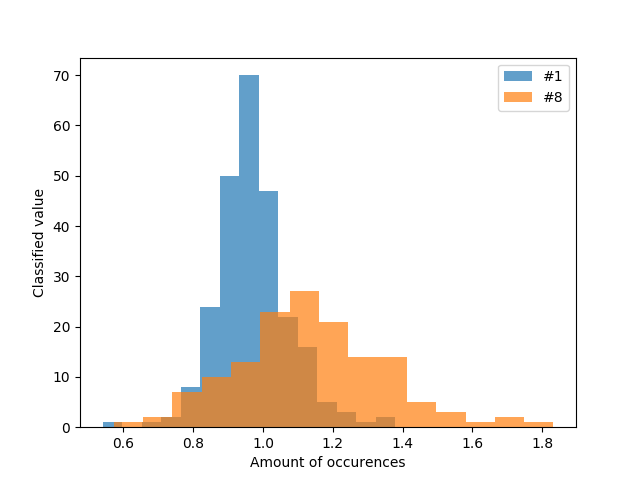
\includegraphics[width=0.9\linewidth]{img/histogram.png}
\caption{Histogram for identifying Digit 1 and Digit 8 based on our selected feature.}
\label{fig:histogram}
\end{figure}

\section{Exercise 4: Multiclass Perceptron}
%Train your network on the train set and evaluate on both the train and the test set, in the same way as you did in the previous steps%
We implemented the net as specified and let it run till it reaches a 100\% accuarcy on the training set. This will surely lead to overfitting.
It takes around 230 to 300 iterations until the weights for the training set results in 100\% accuracy.
When applying the net to the test set we achieved an accuracy of 0.86\%.
Our resulting confusion matrix can be seen in Figure \ref{fig:cmperceptron}. It shows that the numbers hardest to classify seem to be 5 and 4.
\begin{figure}[H]
\centering
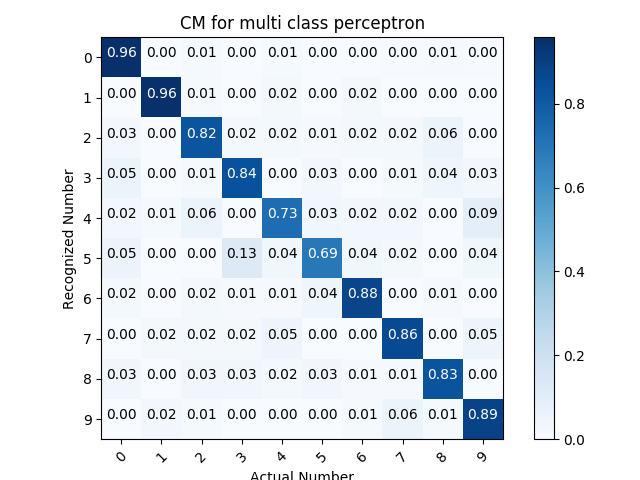
\includegraphics[width=0.9\linewidth]{img/cmperceptron.png}
\caption{Histogram for identifying Digit 1 and Digit 8 based on our selected feature.}
\label{fig:cmperceptron}
\end{figure}

\section{Excercise 5: Gradient Descent}
%monitor two values: the MSE made by your network on the training set (it should be dropping), and the number of misclassified inputs.%
%alternative functions tanh, relu%
%using various initialization strategies and values of the learning rate%
In order to monitor the MSE for the different activation functions we decided to plot a line chart where on the x-axis the amount of iterations and on the y-axis the MSE is portrayed. We purposely did not include the initial MSE, because it heavily drops after the first iteration. This is especially true for the \emph{hyperbolic tangent} which sometimes starts at $MSE=100$.

Other possible conclusions include that the \emph{sigmoid} function benefits from a learning rate $r>0.1$ where as the \emph{linear rectifier} and \emph{hyperbolic tangent} are better if the learning rate $r\leq1$.

Given the evaluation graphs we can conclude that the \emph{sigmoid} activation function performs best if the learning rate is very high (e.g. 4) and the weights are initialized randomly (see Figure \ref{fig:mser4}).  Here we almost reach an MSE of 0.

The \emph{linear rectifier} activation function usually produces very bad results, except if the learning rate is 0.1 and the weights are initialized randomly where it almost reaches an MSE of 0 (see Figure \ref{fig:mser01}).

The \emph{hyperbolic tangent} activation function is quite unpredictable. Usually it produces very bad results, or jitters heavily per iteration (see Figure \ref{fig:mser05}). Although at one point it reaches the very best value of around 0.4, it immediately jitters back and in the end it stays at an MSE of 1.5 which is very bad.
The best stable result we were able to achieve is with a learning rate of 0.1 and weights initialized randomly.

% try more learning rates%

%all random%
\begin{figure}[H]
\centering
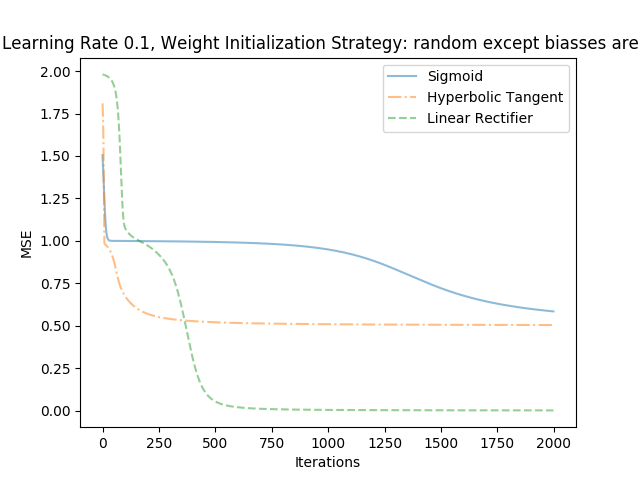
\includegraphics[width=0.9\linewidth]{img/mse_randomexceptbiassesare1_01.png}
\caption{MSE evolution with all weights initialized randomly and learning rate 0.1}
\label{fig:mser01}
\end{figure}
\begin{figure}[H]
\centering
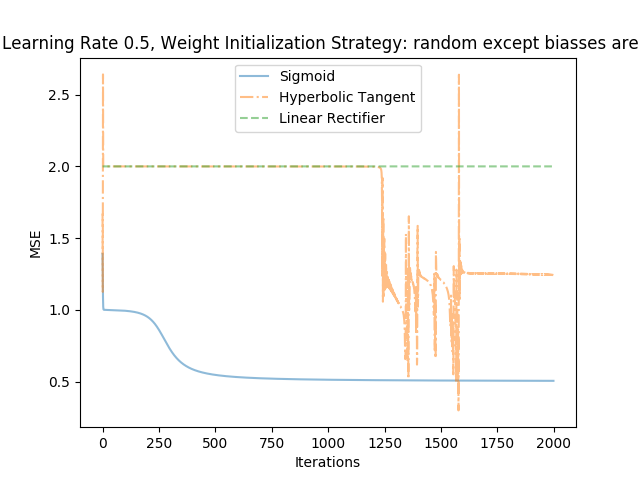
\includegraphics[width=0.9\linewidth]{img/mse_randomexceptbiassesare1_05.png}
\caption{MSE evolution with all weights initialized randomly and learning rate 0.5}
\label{fig:mser05}
\end{figure}
\begin{figure}[H]
\centering
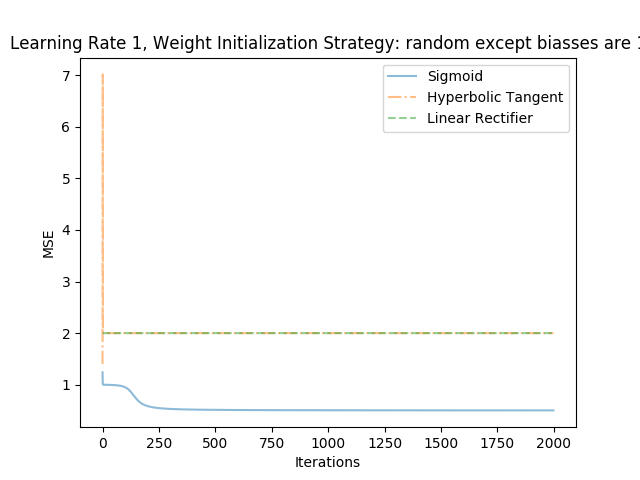
\includegraphics[width=0.9\linewidth]{img/mse_randomexceptbiassesare1_1.png}
\caption{MSE evolution with all weights initialized randomly and learning rate 1}
\label{fig:mser1}
\end{figure}
\begin{figure}[H]
\centering
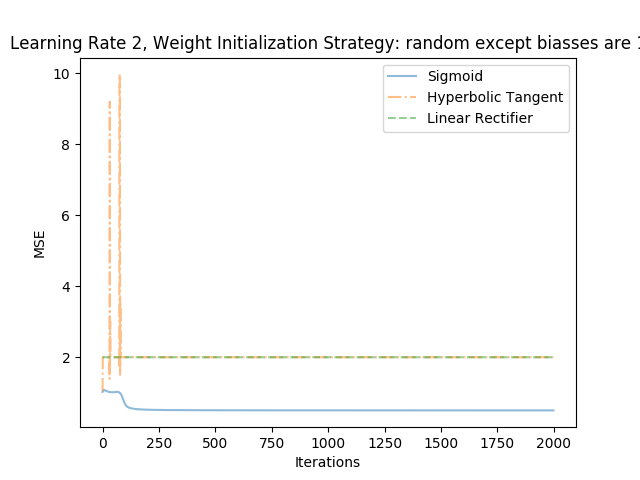
\includegraphics[width=0.9\linewidth]{img/mse_randomexceptbiassesare1_2.png}
\caption{MSE evolution with all weights initialized randomly and learning rate 2}
\label{fig:mser2}
\end{figure}
\begin{figure}[H]
\centering
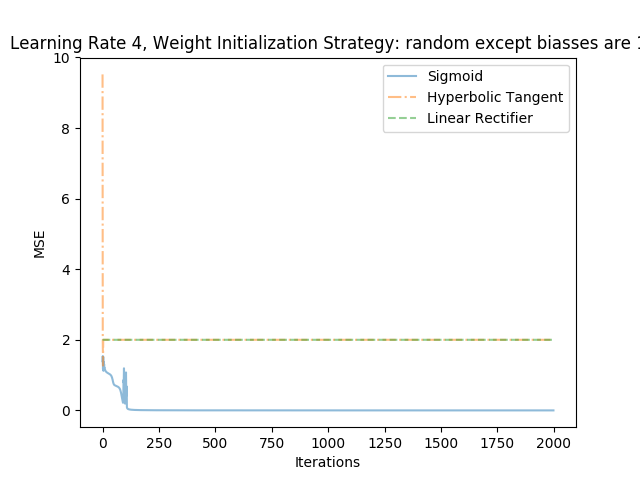
\includegraphics[width=0.9\linewidth]{img/mse_randomexceptbiassesare1_4.png}
\caption{MSE evolution with all weights initialized randomly and learning rate 4}
\label{fig:mser4}
\end{figure}


%all 05 %
\begin{figure}[H]
\centering
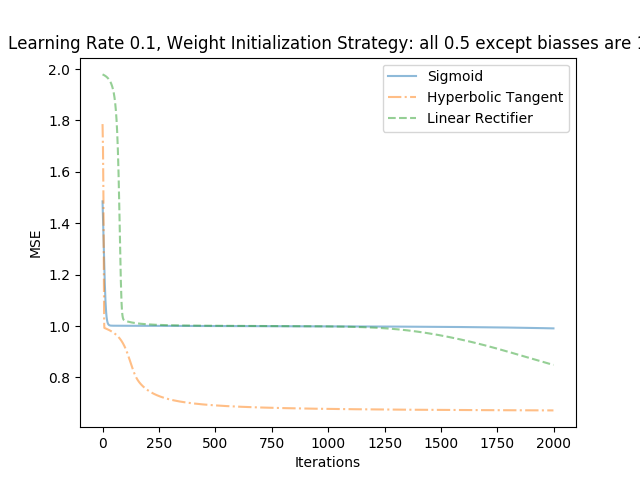
\includegraphics[width=0.9\linewidth]{img/mse_all05exceptbiassesare1_01.png}
\caption{MSE evolution with all weights set to 0.5 and learning rate 0.1}
\label{fig:mse0501}
\end{figure}
\begin{figure}[H]
\centering
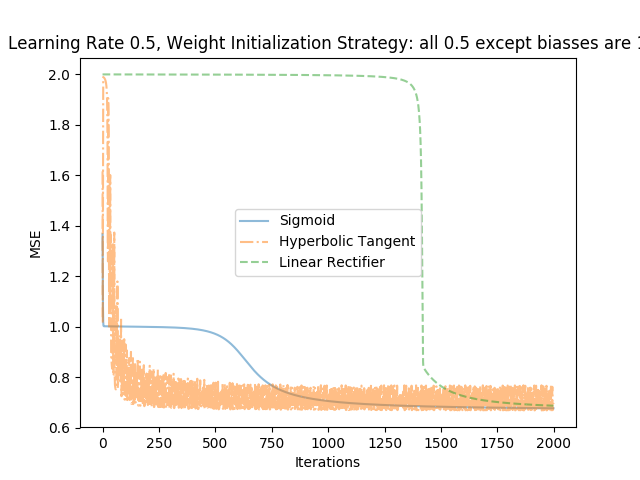
\includegraphics[width=0.9\linewidth]{img/mse_all05exceptbiassesare1_05.png}
\caption{MSE evolution with all weights set to 0.5 and learning rate 0.5}
\label{fig:mse0505}
\end{figure}
\begin{figure}[H]
\centering
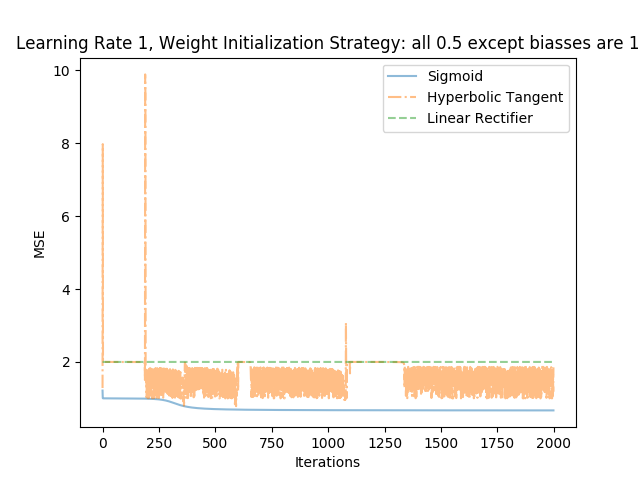
\includegraphics[width=0.9\linewidth]{img/mse_all05exceptbiassesare1_1.png}
\caption{MSE evolution with all weights set to 0.5 and learning rate 1}
\label{fig:mse051}
\end{figure}
\begin{figure}[H]
\centering
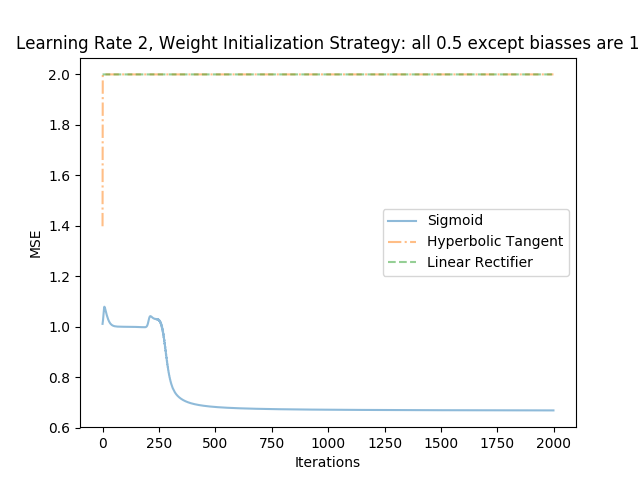
\includegraphics[width=0.9\linewidth]{img/mse_all05exceptbiassesare1_2.png}
\caption{MSE evolution with all weights set to 0.5 and learning rate 2}
\label{fig:mse052}
\end{figure}
%all 1 %
\begin{figure}[H]
\centering
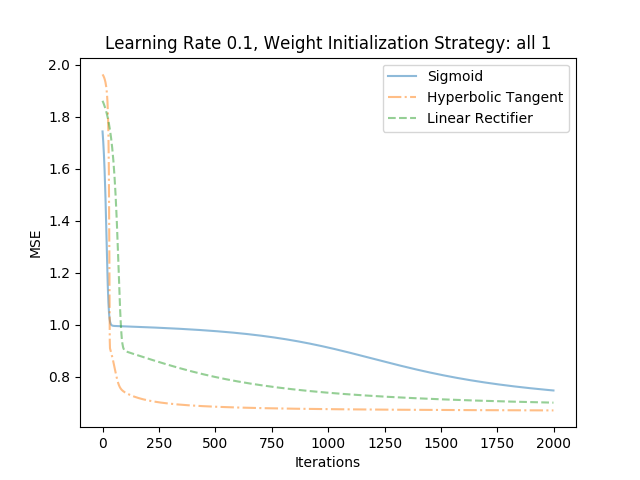
\includegraphics[width=0.9\linewidth]{img/mse_all1_01.png}
\caption{MSE evolution with all weights set to 1 and learning rate 0.1}
\label{fig:mse101}
\end{figure}
\begin{figure}[H]
\centering
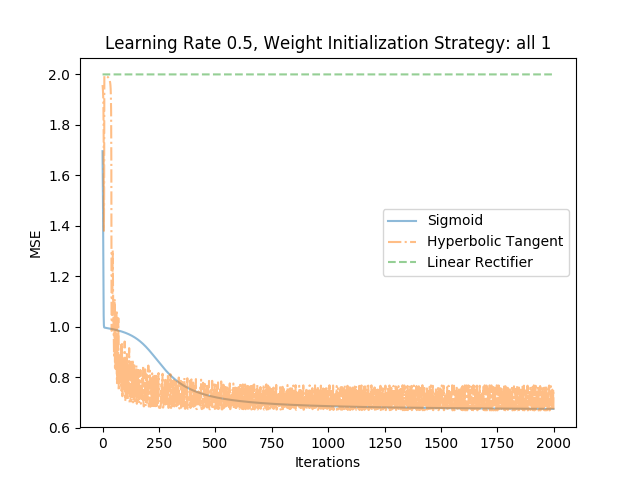
\includegraphics[width=0.9\linewidth]{img/mse_all1_05.png}
\caption{MSE evolution with all weights set to 1 and learning rate 0.5}
\label{fig:mse105}
\end{figure}
\begin{figure}[H]
\centering
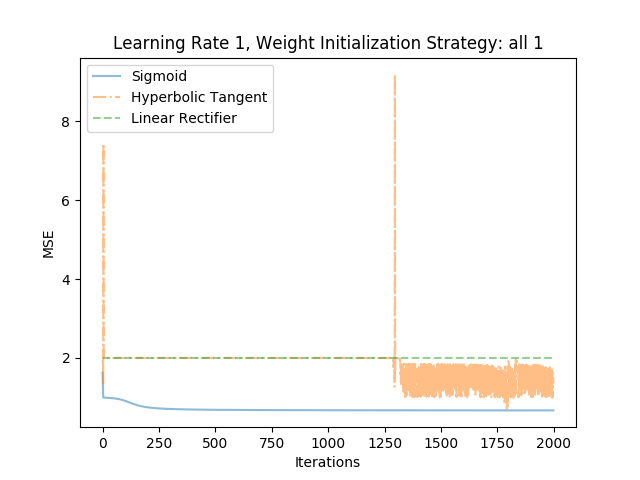
\includegraphics[width=0.9\linewidth]{img/mse_all1_1.png}
\caption{MSE evolution with all weights set to 1 and learning rate 1}
\label{fig:mse11}
\end{figure}
\begin{figure}[H]
\centering
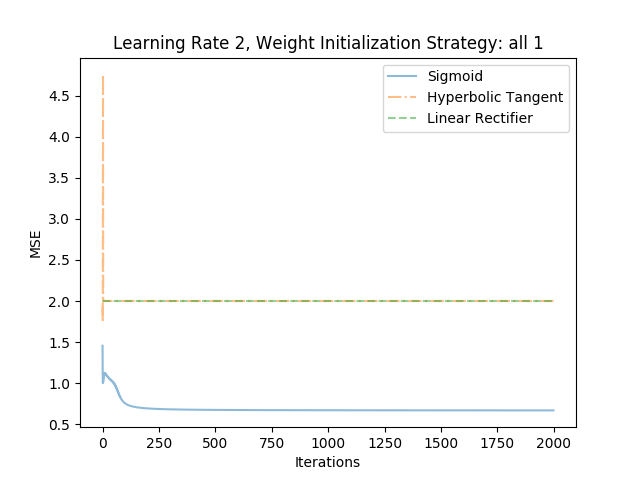
\includegraphics[width=0.9\linewidth]{img/mse_all1_2.png}
\caption{MSE evolution with all weights set to 1 and learning rate 2}
\label{fig:mse12}
\end{figure}
\begin{figure}[H]
\centering
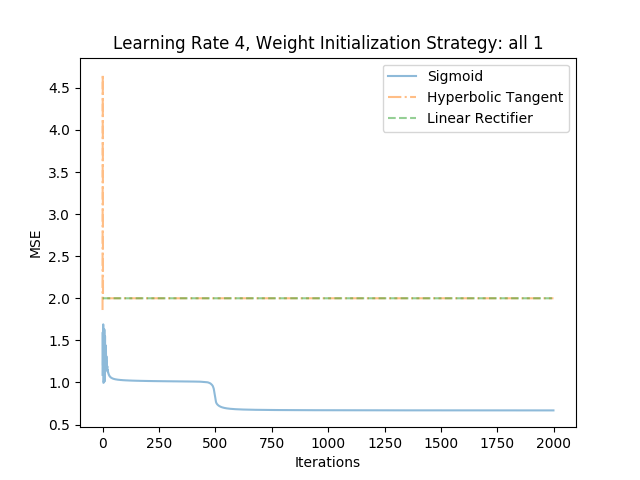
\includegraphics[width=0.9\linewidth]{img/mse_all1_4.png}
\caption{MSE evolution with all weights set to 1 and learning rate 4}
\label{fig:mse14}
\end{figure}
%all 0%
\begin{figure}[H]
\centering
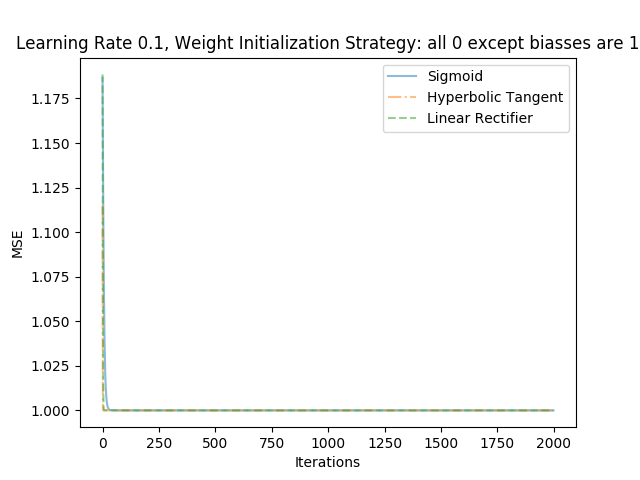
\includegraphics[width=0.9\linewidth]{img/mse_all0exceptbiassesare1_01.png}
\caption{MSE evolution with all weights set to 0 and learning rate 0.1}
\label{fig:mse201}
\end{figure}
\begin{figure}[H]
\centering
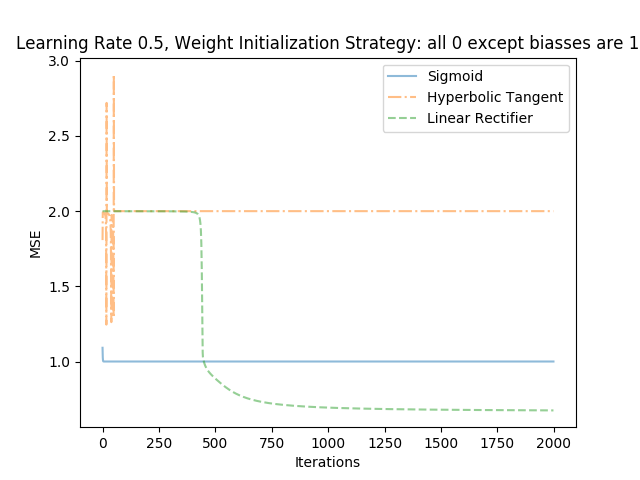
\includegraphics[width=0.9\linewidth]{img/mse_all0exceptbiassesare1_05.png}
\caption{MSE evolution with all weights set to 0 and learning rate 0.5}
\label{fig:mse205}
\end{figure}
\begin{figure}[H]
\centering
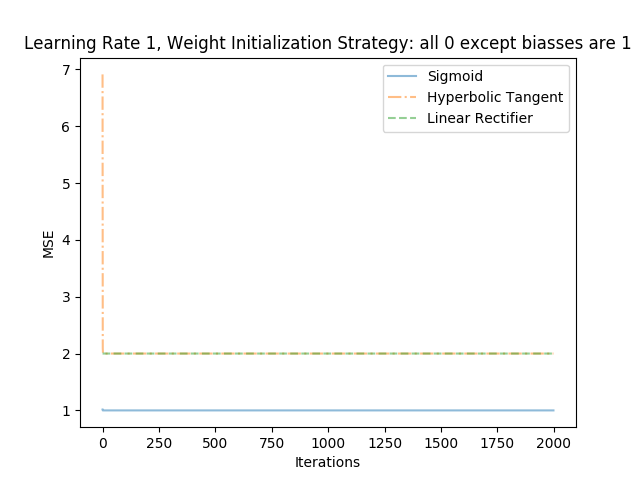
\includegraphics[width=0.9\linewidth]{img/mse_all0exceptbiassesare1_1.png}
\caption{MSE evolution with all weights set to 0 and learning rate 1}
\label{fig:mse12}
\end{figure}
\begin{figure}[H]
\centering
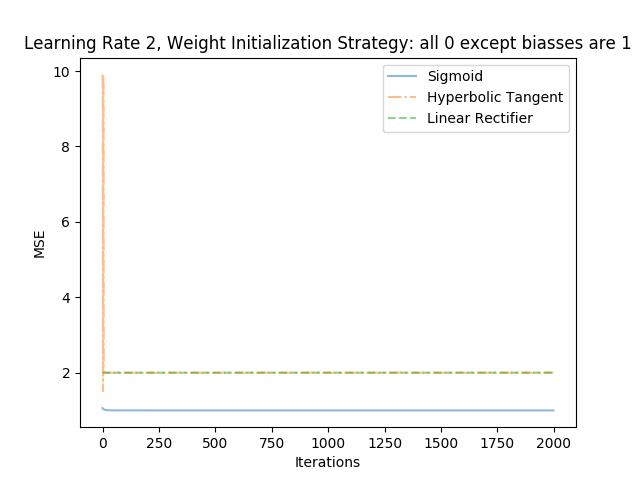
\includegraphics[width=0.9\linewidth]{img/mse_all0exceptbiassesare1_2.png}
\caption{MSE evolution with all weights set to 0 and learning rate 2}
\label{fig:mse22}
\end{figure}
\begin{figure}[H]
\centering
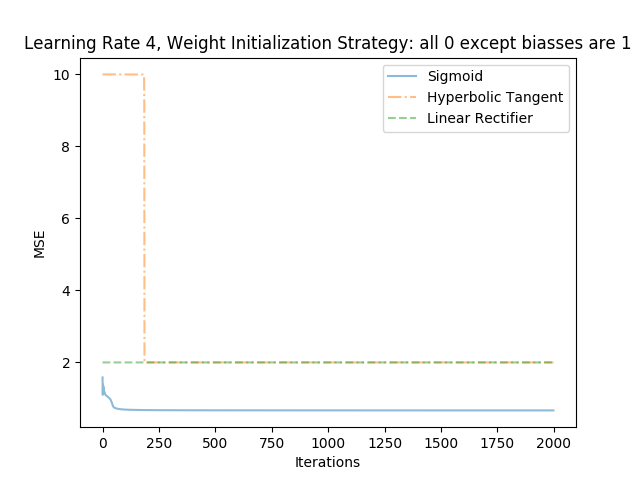
\includegraphics[width=0.9\linewidth]{img/mse_all0exceptbiassesare1_4.png}
\caption{MSE evolution with all weights set to 0 and learning rate 4}
\label{fig:mse24}
\end{figure}



\end{document}